%%%%%%%%%%%%%%%%%%%%%%% file template.tex %%%%%%%%%%%%%%%%%%%%%%%%%
%
% This is a general template file for the LaTeX package SVJour3
% for Springer journals.          Springer Heidelberg 2010/09/16
%
% Copy it to a new file with a new name and use it as the basis
% for your article. Delete % signs as needed.
%
% This template includes a few options for different layouts and
% content for various journals. Please consult a previous issue of
% your journal as needed.
%
%%%%%%%%%%%%%%%%%%%%%%%%%%%%%%%%%%%%%%%%%%%%%%%%%%%%%%%%%%%%%%%%%%%
%
% First comes an example EPS file -- just ignore it and
% proceed on the \documentclass line
% your LaTeX will extract the file if required
\begin{filecontents*}{example.eps}
%!PS-Adobe-3.0 EPSF-3.0
%%BoundingBox: 19 19 221 221
%%CreationDate: Mon Sep 29 1997
%%Creator: programmed by hand (JK)
%%EndComments
gsave
newpath
  20 20 moveto
  20 220 lineto
  220 220 lineto
  220 20 lineto
closepath
2 setlinewidth
gsave
  .4 setgray fill
grestore
stroke
grestore
\end{filecontents*}
%
\RequirePackage{fix-cm}
%
%\documentclass{svjour3}                     % onecolumn (standard format)
%\documentclass[smallcondensed]{svjour3}     % onecolumn (ditto)
\documentclass[smallextended]{svjour3}       % onecolumn (second format)
%\documentclass[twocolumn]{svjour3}          % twocolumn
%
\smartqed  % flush right qed marks, e.g. at end of proof
%
\usepackage{graphicx}
\usepackage{varwidth}
\usepackage{setspace}
\usepackage{perpage}
\usepackage{enumerate}
\MakePerPage{footnote}
%
% \usepackage{mathptmx}      % use Times fonts if available on your TeX system
%
% insert here the call for the packages your document requires
%\usepackage{latexsym}
% etc.
%
% please place your own definitions here and don't use \def but
% \newcommand{}{}
%
% Insert the name of "your journal" with
% \journalname{myjournal}
%

\raggedbottom

\begin{document}

\title{Toward Improving Human-Robot Collaboration with Emotional Awareness}%\thanks{Grants or
% other notes about the article that should go on the front page should be
%placed here. General acknowledgments should be placed at the end of the article.}
%}

%\subtitle{Do you have a subtitle?\\ If so, write it here}

%\titlerunning{Short form of title}        % if too long for running head

\author{Mohammad Shayganfar \and
        Charles Rich \and
        Candace L. Sidner
}

%\authorrunning{Short form of author list} % if too long for running head

\institute{Mohammad Shayganfar \and Charles Rich \and Candace L. Sidner \at
              100 Institute Road, Worcester, MA, USA 01609-2280 \\
              Tel.: +1 508-831-5357\\
              Fax: +1 508-831-5776\\
              \email{mshayganfar@wpi.edu}\\
              \email{rich@wpi.edu}\\
              \email{sidner@wpi.edu}\\
%             \emph{Present address:} of F. Author  %  if needed
}

\date{Received: date / Accepted: date}
% The correct dates will be entered by the editor


\maketitle

\begin{abstract}

Current computational theories for human-robot collaboration specify the
structure of collaborative activities, but are weak on the underlying processes
that generate and maintain these structures.  We argue that emotions are crucial
to these underlying processes and have developed a new computational theory,
called \textit{Affective Motivational Collaboration Theory}, that combines
emotion-based processes, such as appraisal and coping, with collaboration
processes, such as planning, in a single unified framework. To illustrate the
application of this new theory, we present detailed computational walkthroughs
contrasting the behavior of an emotionally aware robot with an emotionally
ignorant robot in the same situations.  These walkthroughs are the starting
point for our implementation of the theory. 

\keywords{Human-Robot Collaboration \and Emotional-Awareness \and Affective
Motivational Collaboration Theory}
% \PACS{PACS code1 \and PACS code2 \and more}
% \subclass{MSC code1 \and MSC code2 \and more}
\end{abstract}

\section{Introduction}
\label{intro}

A key aspect of the sociability of robots will be their ability to collaborate
with humans in the same environment. Collaboration is a coordinated activity in
which the participants work jointly to satisfy a shared goal
\cite{grosz:plans-discourse}. There are many challenges in achieving a
successful collaboration between robots and humans. To meet this challenges, it
is crucial to understand what makes a collaboration not only successful, but
also efficient. Existing computational models of collaboration explain some of
the important concepts underlying collaboration; such as the presence of a
reason for collaborators' commitment, and the necessity of communicating about
mental states in order to maintain progress over the course of a collaboration.
The most prominent collaboration theories are based on plans and intentions
\cite{cohen:teamwork} \cite{grosz:plans-discourse}
\cite{Litman:discourse-commonsense}, and are derived from Bratman's BDI
architecture \cite{bratman:intentions-plans}. Two theories, Joint Intentions
\cite{cohen:teamwork} and SharedPlans
\cite{grosz:planning-acting,grosz:collaboration,grosz:plans-discourse}, have
been used to support teamwork and collaboration between humans and robots or
virtual agents \cite{breazeal:humanoid-robots}
\cite{montreuil:planning-robot-activity} \cite{sidner:enagagement-robot}
\cite{yen:cast}. However, these theories explain only the structure of a
collaboration. For instance, in SharedPlans theory collaborators build a shared
plan containing a collection of beliefs and intentions about the actions in the
plan. Collaborators communicate these beliefs and intentions via utterances
about actions that contribute to the shared plan. This communication leads to
the incremental construction of a shared plan, and ultimately successful
completion of the collaboration. In contrast, in Joint Intentions theory, the
notion of joint intention is viewed as a persistent commitment of the team
members to a shared goal. In this theory, once an agent enters into a joint
commitment with other agents, it should communicate its private beliefs to other
team members.

Although existing collaboration theories explain the important elements of a
collaboration structure, the underlying processes required to dynamically
create, use, and maintain the elements of this structure are largely
unexplained. For instance, a general mechanism has yet to be developed that
allows an agent to effectively integrate the influence of its collaborator's
perceived or anticipated emotions into its own cognitive mechanisms to prevent
shared task failures while maintining collaborative behavior. Therefore, a
process view of collaboration must include certain key elements. It should
inherently involve social interactions since all collaborations occur between
social agents, and it should essentially constitute a means of modifying the
content of social interaction as the collaboration unfolds. The underlying
processes of emotions possess these two properties, and social functions of
emotions explain some aspects of the underlying processes in collaboration. This
paper makes the case for a process model of emotions and demonstrates how it
furthers collaboration between humans and robots.

Humans are emotional and social beings; emotions are involved in many different
social contexts including collaboration. Although there are purely personal
emotions, most emotions are importantly experienced in a social context and
acquire their significance in relation to this context
\cite{parkinson:emotion-social-interaction}. For instance, humans are influenced
by the emotions of those around them. They also have emotions about the actions
of people around them. They have emotions about the events that occur in the other
people's lives. Also, humans' concern about their relationships with others
elicits emotion. They can feel emotion about their personal successes and
failures and those of others. Moreover, socially shared and regulated emotions
can provide social meanings to events happening in the environment
\cite{wisecup:sociology-emotions}. 

There is also a communicative aspect of emotions. For instance, emotions are
often intended to convey information to others \cite{goffman:self-presentation}.
Emotions are also involved in verbal behaviors. For instance, an utterance can
include both content and relational meaning. An emotion might appear to be
elicited by the content of the utterance, but in fact be an individual's
response to the relational meaning \cite{planalp:communicating-emotion}. The
interpretation of these relational meanings are handled by the appraisal of
events. Appraisal processes give us a way to view emotion as social
\cite{hooft:sharing-emotions}. Meaning is created by an individual's social
relationships and experiences in the social world, and individuals communicate
these meanings through utterances. Consequently, the meaning of these utterances
and the emotional communication change the dynamic of social interactions. A
successful and effective emotional communication necessitates ongoing reciprocal
adjustments between interactants that can happen by interpreting each other's
behaviors \cite{parkinson:emotion-social-interaction}. This adjustment procedure
requires a baseline and an assessment procedure. While the components of the
collaboration structure, e.g., shared plan, provide the baseline,
emotion-related processes provide the assessment procedure.

Since collaboration is a type of social context, the social functions of
emotions are required for an agent to perform adequately in such an environment.
In this paper, we present two pairs of hypothetical interaction scenarios. Each
pair contrasts an emotionally-aware with an emotionally-ignorant robot
iteracting with a human in the same situation. These scenarios highlight the
necessity of giving robots the capacity to understand and regulate emotions, as
well as to provide emotion-driven responses. We then briefly introduce
\textit{Affective Motivational Collaboration Theory} which explains the
underlying processes of emotions and collaboration. The emotion-aware examples
show how the mechanisms of this theory are involved in agreeing on a shared goal
with a robot (Sections \ref{sec:exp1} and \ref{sec:wt-exp1}), and delegating a
new task to the robot (Sections \ref{sec:exp3} and \ref{sec:wt-exp3}). The
emotion-ignorance examples are the same, except that the robot ignores the
human's verbally or nonverbally expressed emotions. The same four examples in
Sections \ref{sec:exp1} to \ref{sec:exp4} are revisited in more detail in our
computational walkthroughs in Section \ref{sec:wtce}. In this section, we show
how the mechanisms of \textit{Affective Motivational Collaboration Theory}
operate to produce the robot behaviors in Section \ref{sec:example-scenario}.

As we discussed above, there are certain types of emotion-regulated mechanisms
with which a collaborative robot can modify and maintain a collaboration
structure (e.g., shared plan). We explain these mechanisms and their
corresponding operations in \textit{Affective Motivational Collaboration
Theory}. In this paper, we briefly describe some parts of this theory that are
required to discuss our examples. We have also implemented all the rules
asscoiated with each mechanism using JESS (JAVA Expert System Shell) to be able
to generate the same type of collaborative behaviors as they appear in our
examples. In the future, we are going to use these rules and the processes
involved in each mechanism to build collaborative behaviors in an interactive
robot.

\section{Example Scenarios}
\label{sec:example-scenario}
%Text with citations \cite{RefB} and \cite{RefJ}.

\subsection{Backstory}

The scenarios transpire in a lunar facility using collaborative robots to work
with astronauts. The mission is to finish installing the solar panels required
to provide energy for the operation of the facility. Most of the panels have
already been installed. However, the facility is now faced with a low batteries
situation, which forces the team to be cautious about consuming energy. A female
astronaut is inspecting the working conditions in the field and planning the
installation of the remaining panels in collaboration with the robot.

\subsection{Astronaut-Robot Interaction}

The Robot and the Astronaut will collaborate with each other to achieve their
shared goal, which is to install two solar panels. They will face various
difficulties, ranging from the task being unpleasant and challenging to
conflicts of their private and/or shared goals because of a blocked or a
protracted sub-task. The Robot and the Astronaut will go through a series of
assessment processes to figure out a) how did the current blockage happen? b)
why is the current task is blocked? and c) what is the next action they are
going to take? The robot uses its cognitive abilities and communication skills
to overcome these problems, to motivate the astronaut, and to propose
alternative tasks. The following is part of an interaction between the Astronaut
and the Robot during their collaboration on installing solar panels.

\subsection{Agreeing on Shared Goal (Emotion-Awareness)}
\label{sec:exp1}

This hypothetical example and the emotion-ignorant version in the next section
demonstrate that agreeing on a shared goal requires the Robot to be aware of its
collaborator's emotions (here, frustration). 

\begin{description}
  \item \textit{\textbf{\fontsize{9pt}{12pt}\selectfont{A1. Astronaut:}}} Oh
  no! Finishing the quality check of our installation with this measurement
  problem is so frustrating. I think we should stop now!\\

  \item \fbox{\begin{varwidth}{0.96\textwidth}
  \textit{\textbf{\fontsize{9pt}{12pt}\selectfont{A2. Robot:}}} \underline{I
  see. This is frustrating.} But, I can help you with the measurement tool and
  we can finish the task as originally planned.
  \end{varwidth}}\\
  
  \item \textit{\textbf{\fontsize{9pt}{12pt}\selectfont{A3. Astronaut:}}} Can
  you fix the measurement tool?\\

  \item \textit{\textbf{\fontsize{9pt}{12pt}\selectfont{A4. Robot:}}} The next
  task is fixing the panel and it requires you to prepare and attach the welding
  rod to your welding tool. To save our time, I will fetch another measurement
  tool while you are preparing your welding tool.\\

  \item \textit{\textbf{\fontsize{9pt}{12pt}\selectfont{A5. Astronaut:}}} That
  would be great!
  
\end{description}

The Astronaut's first turn (A1), shows her verbally conveying her frustration
with respect to a malfunctioning measurement tool that is used for checking the
quality of the installed panel. In reply, the Robot's first turn (A2) shows the
Robot perceiving the Astronaut's frustration and acknowledging it verbally. The
underlined section of the Robot's utterances (in turn A2) shows the influence of
using emotion-driven processes which leads to acknowledgement of the Astronaut's
emotion. See the absence of these utterances as the consequence of ignoring the
Astronaut's emotions in the same turn in the next example (Section
\ref{sec:exp2}). In Section \ref{sec:wt-exp1}, we will show how the
computational mechanisms discussed in Section \ref{sec:AMCT} are involved in
this process, specifically how these emotion-driven goal-directed mechanisms
work together and lead to the Robot's behavior acknowledging the perceived
emotion of the Astronaut properly, thereby avoiding unsuccessful termination of
the collaboration.

Continuing in turn A3, the Astronaut's utterance shows a change of underlying
belief from termination of the collaboration to the possibility of seeking
instrumental support by asking the Robot whether it is possible to fix the
measurement tool. Notice that the proper acknowledgement of the Astronaut's
emotion helps to change her emotion from frustration to neutral. Now that in A3
the Astronaut is no longer expressing a negative emotion (i.e., frustration),
and is asking for help, the Robot can provide an alternative task as a potential
solution (A4). This illustrates an advantage of emotional-awareness: Although
the Robot, according to the shared plan, could have provided the same
alternative task as a solution to the Astronaut immediately, it delayed instead,
providing the potential solution after first dealing with the Astronaut's
negative emotional state. Finally, since agreeing on a shared goal is a
collaborative negotiation process, emotion-awareness plays a crucial role in
providing a fair offer. As a result, the Astronaut's response in the last turn
(A5) shows acceptance and contentment with the Robot's potential solution to
continue collaboration and agreement on the shared goal.

In the next example we show what happens in the same hypothetical situation when
the Robot ignores the Astronaut's emotion and tries to save the collaboration
process from failure.

\subsection{Agreeing on Shared Goal (Emotion-Ignorance)}
\label{sec:exp2}

This example shows the same process of agreeing on a shared goal as in the
previous section except that it diverges from reaching an agreement, despite the
fact that it begins with the same utterance (B1) as the previous example (A1). 

\begin{description}
  \item \textit{\textbf{\fontsize{9pt}{12pt}\selectfont{B1. Astronaut:}}} Oh no!
  Finishing the quality check of our installation with this measurement problem
  is so frustrating. I think we should stop now!\\

  \item \fbox{\begin{varwidth}{0.96\textwidth}
  \textit{\textbf{\fontsize{9pt}{12pt}\selectfont{B2. Robot:}}} I can help you
  with the measurement tool, or we can terminate this task.
  \underline{What do you want me to do?}\end{varwidth}}\\
  
  \item \textit{\textbf{\fontsize{9pt}{12pt}\selectfont{B3. Astronaut:}}} As I
  said the measurement tool does not work properly. We can not continue!\\

  \item \textit{\textbf{\fontsize{9pt}{12pt}\selectfont{B4. Robot:}}} Okay. Do
  you want me to fix this problem or terminate the task?\\

  \item \textit{\textbf{\fontsize{9pt}{12pt}\selectfont{B5. Astronaut:}}} Can
  you fix my measurement tool?\\
  
  \item \textit{\textbf{\fontsize{9pt}{12pt}\selectfont{B6. Robot:}}} I cannot
  fix your measurement tool, but I can fetch another one for you if you want?\\
  
  \item \textit{\textbf{\fontsize{9pt}{12pt}\selectfont{B7. Astronaut:}}} No, I
  don't want another measurement tool! We don't have time for that!\\
  
  \item \fbox{\begin{varwidth}{0.96\textwidth}
  \textit{\textbf{\fontsize{9pt}{12pt}\selectfont{B8. Robot:}}} Okay.
  You want me to terminate this task. Terminating this task can influence the
  quality of installation of this solar panel which can cause the mission to
  fail. Or, \underline{do you want us to work on another task?} This can help us
  to install the panel using your welding tool, but I do not know whether the
  quality of our installation will be acceptable.\end{varwidth}}\\
  
  \item \textit{\textbf{\fontsize{9pt}{12pt}\selectfont{B9. Astronaut:}}} I told
  you we have this problem and we should terminate the mission! We cannot
  continue without the measurement tool!
\end{description}

As mentioned earlier, emotional-awareness is beneficial in collaboration by
channeling the collaboration process towards the shared goal. Without
emotional-awareness a collaborative Robot will try to maintain the status of the
shared goal and prevent it from failure without considering its collaborator's
negative emotion which can be the result of the task failure. In this example,
the emotionally-ignorant Robot does not acknowledge the Astronaut's frustration
(compare B2 with A2 above), since it does not perceive that emotion. Then, while
negotiating the shared goal the Robot fails to offer a potential solution with
respect to the Astronaut's emotional state. As a result, it causes the failure
of the negotiation procedure during collaboration.

The Robot, in this example, does not perceive the Astronaut's emotion, since it
does not apply the Astronaut's emotion (frustration) as an influential factor in
its computational mechanisms (see details in Section
\ref{sec:computational-framework}). Hence, in the Robot's first response (B2),
it does not acknowledge the Astronaut's emotion, and instead immediately conveys
two available alternative actions according to the existing shared plan, and
asks the Astronaut to select between them. As shown in the Astronaut's response
(B3), the Robot's immediate proposal does not result in any progress in
collaboration. As a result, the Astronaut repeats herself about the task status
while still expressing frustration. The Astronaut's response does not change the
Robot's mental state and this causes the Robot to try to repeat its own question
while still missing the Astronaut's frustration (B4). The Robot's utterance
creates an ambiguous assumption for the Astronaut about whether the Robot can
fix the broken measurement tool for her. This ambiguity makes the Astronaut even
more frustrated and causes her to ask a question to remove the ambiguity of the
Robot's proposal (B5). In return, the Robot not only misses the Astronaut's
intensified frustration, but also nullifies the Astronaut's assumption about
fixing the disfunctional measurement tool and proposes the potential solution of
replacing the broken tool and asking whether the Astronaut agrees on that (B6).

In B7, the Astronaut modifies its assumption and announces the shortage of time
as justification for expressing her anger. At this point, the Robot's response
becomes more crucial since its wrong method of interaction and
emotionally-ignorant behavior shifted the Astronaut's emotional and mental
states into a noncollaborative status. Consequently, the Robot again attempts to
revive the collaboration process, and therefore it provides more information
about the repercussions of terminating the collaboration process, to see whether
the Astronaut can pursue another task (B8). Notice the underlined section of the
Robot's turn B8 indicates its dissociated reasoning about the problem from the
Astronaut's mental state. Finally, the poor interaction of the Robot caused by
its emotionally-ignorant behavior which developed from the Robot's very first
response and has continued till the end, leads to an unsuccessful termination of
their collaboration (B9).\\

\subsection{Task Delegation (Emotion-Awareness)}
\label{sec:exp3}

In this and the next section, a different collaborative behavior, task
delegation, is used to illustrate how collaboration critically depends on
understanding how worried the other collaborator is. This example shows that
when the Robot is aware of the Astronaut's worry, it can use its own motivation
mechanism driven by emotions to come up with a way to alleviate her worry. Its
solution is to postpone all questions until such time as they are
critical. 

\begin{description}
  \item \textit{\textbf{\fontsize{9pt}{12pt}\selectfont{C1. Astronaut:}}} I
  still have some problems with attaching the first panel! We do not have enough
  time. You should begin to install the second panel.\\

  \item \fbox{\begin{varwidth}{0.96\textwidth}
  \textit{\textbf{\fontsize{9pt}{12pt}\selectfont{C2. Robot:}}} Okay.
  \underline{Don't worry.} I can handle that.\end{varwidth}}\\

  \item \textit{\textbf{\fontsize{9pt}{12pt}\selectfont{C3. Astronaut:}}} I will
  try to fix it asap.\\

  \item \textit{\textbf{\fontsize{9pt}{12pt}\selectfont{C4. Robot:}}} I might
  need to ask some questions while I am installing the second panel.\\

  \item \textit{\textbf{\fontsize{9pt}{12pt}\selectfont{C5. Astronaut:}}} That's
  fine. Just let me know.
  
\end{description}

At the beginning of this example Astronaut (C1) is worried because of the lack
of time to achieve the shared goal (finishing installation of solar panels). She
proposes that the Robot begin installing the second panel, since the first one
still has some problems. The Robot in its first turn (C2), perceives the
Astronaut's emotion (i.e., worry) and, using the same cognitive mechanisms (see
Section \ref{sec:AMCT}), acknowledges the Astronaut's emotion just as it did in
first example in Section \ref{sec:exp1}. The underlined utterance in the Robot's
turn C2, shows the Robot's awareness of the Astronaut's emotion. Also, the Robot
does not ask the Astronaut (because of perceiving her worry) if it is okay to
leave the current task which was helping the Astronaut to install the first
panel. Because the Robot knows that redirecting the Astronaut's attention away
from the object of worry will create frustration, as the function of worry is to
resolve the object of worry.

After acknowledging the Astronaut's emotion (C2), the Robot infers that it needs
to postpone asking questions about the missing parts of the shared plan since
installing a panel is a collaborative task and some of the primitive tasks need
to be done by the Astronaut. Then, the Astronaut perceives the Robot's response
as a proper acceptance of the task delegation and tries to communicate the
status of her own task, even though she is still worried about finishing the
overall task (C3). Now, the Robot perceives the Astronaut's worry and without
asking the actual detailed questions about the delegated task, declares the
possibility of asking some follow-up questions whenever the Astronaut's answers
are required to make progress in executing some primitive tasks while installing
the second panel (C4). Thus, the Robot not only prevents overwhelming the
Astronaut with several questions related to executing the next steps in the
future, but its utterance implicitly reveals its knowledge of tasks'
requirements to the Astronaut. As a result, the Robot's approach to acceptance
of the delegated task mitigates the Astronaut's negative emotion (i.e., worry)
which makes her to respond positively to the Robot's proposal.

The next section shows the same task delegation situation with the negative
impact of the Robot ignoring the Astronaut's emotion.

\subsection{Task Delegation (Emotion-Ignorance)}
\label{sec:exp4}

This last example illustrates how ignoring the collaborator's emotions in a task
delegation procedure can negatively impact the progress of a collaboration. In
this example, the emotionally-ignorant Robot is planning in its most efficient
manner (because time is short) and therefore asking a lot of questions so that
it can work out the plan. But asking questions exacerbates the Astronaut's worry
which leads to an unsuccessful collaboration due to the lack of time.

\begin{description}
  \item \textit{\textbf{\fontsize{9pt}{12pt}\selectfont{D1. Astronaut:}}} I
  still have some problems with attaching the first panel! We do not have enough
  time. You should begin to install the second panel.\\

  \item \fbox{\begin{varwidth}{0.96\textwidth}
  \textit{\textbf{\fontsize{9pt}{12pt}\selectfont{D2. Robot:}}} Okay. I can
  handle that. \underline{Is it okay if I leave the current task}
  \underline{though?}\end{varwidth}}\\
  
  \item \textit{\textbf{\fontsize{9pt}{12pt}\selectfont{D3. Astronaut:}}} Yes,
  that's fine. I can finish it on my own.\\

  \item \textit{\textbf{\fontsize{9pt}{12pt}\selectfont{D4. Robot:}}} Okay. But
  according to the plan, I need your help when we need to weld the panel. Will
  you be able to help me?\\

  \item \textit{\textbf{\fontsize{9pt}{12pt}\selectfont{D5. Astronaut:}}} Yes, I
  will.\\
  
  \item \textit{\textbf{\fontsize{9pt}{12pt}\selectfont{D6. Robot:}}} We also
  need your welding tool and supplies as well as the measuring tool to install
  the second panel.\\
  
  \item \textit{\textbf{\fontsize{9pt}{12pt}\selectfont{D7. Astronaut:}}} Just
  let me know whenever you need something!\\
  
  \item \fbox{\begin{varwidth}{0.96\textwidth}
  \textit{\textbf{\fontsize{9pt}{12pt}\selectfont{D8. Robot:}}} Thanks. I will.
  \underline{How about the conflict that might occur while} \underline{I am
  trying to fix the second panel?} You are going to need my help at the same
  time.\end{varwidth}}\\
  
  \item \textit{\textbf{\fontsize{9pt}{12pt}\selectfont{D9. Astronaut:}}} Robot,
  I really don't understand what you are talking about!\\
  
  \item \fbox{\begin{varwidth}{0.96\textwidth}
  \textit{\textbf{\fontsize{9pt}{12pt}\selectfont{D10. Robot:}}} \underline{Do
  you want me to provide some examples?} \end{varwidth}}\\

  \item \textit{\textbf{\fontsize{9pt}{12pt}\selectfont{D11. Astronaut:}}} We
  don't have time for this anymore!
  
\end{description}

The very first utterance of the Astronaut above (D1) is the same as the first
utterance in the previous example (C1). The Astronaut is worried and expresses
her worry. However, the Robot does not perceive and consequently does not
acknowledge the Astronaut's emotion. As a result, the Robot responds to the
Astronaut by trying to determine a proper solution for an action selection
problem. The action selection problem is primarily caused by the shift in the
Robot's focus of attention from an unfinished ongoing task (unsatisfied
postconditions) to a new partially known nonprimitive task (i.e., installing the
second panel). Therefore, the Robot immediately tries to confirm leaving the
current unfinished task (D2). Notice the absence of acknowledgment of the
Astronaut's emotion by the Robot in this turn (compare C2 above and D2 here).

This absence of emotion-awareness is the beginning of the failure of the task
delegation process. As we can see, the Robot's response does not mitigate the
Astronaut's worrying about the future of the collaboration. The underlined
section in D2 shows the Robot's need for confirmation of leaving an unfinished
task. Next, the Astronaut tries to help the Robot to select the proper action by
responding positively about the Robot leaving the current task (D3). Now, the
Robot shifts its focus of attention to the new task and uses the Collaboration
mechanism (see Section \ref{sec:AMCT}) to obtain required information such as
task dependencies, existing preconditions and required resources. Subsequently,
the absence of required information and dependencies to the Astronaut's actions
causes the Robot to ask a question about whether the Astronaut will be able to
help in some parts of the task (D4). Although this type of interactive behavior
is crucial in many collaborative contexts, here it is counter productive. Thus,
the Astronaut succinctly responds to the Robot's question while she is still
worried about finishing installation of the first panel (D5). The Robot asks
another question about the required inputs for the task which are dependent on
the Astronaut without considering her worry (D6). At this point, since the
Astronaut believes that the Robot's questions are unnecessary, she becomes
frustrated and impatiently answers the Robot's question (D7). However, once
again, not only does the Robot miss the Astronaut's emotion, but it also wants
to prevent failure of a task in the future (D8). Notice that the underlined
section in D8 is the result of the Robot's inference about the possibility of a
future problem. Also, note that while the Robot is capable of operating based on
a partial plan, instead, the Robot continues to attempt to develop a full plan
due to ignorance of the Astronaut's frustration. Then, the Astronaut does not
recall the event referenced by the Robot and since she is frustrated, she does
not even try to remove the ambiguity of the existing issue (D9). Once again, the
Robot misses the Astronaut's frustration and tries to see whether the Astronaut
wants the Robot to clarify the issue for her by providing her some examples
(D10). The underlined utterance in D10 indicates another situation in which the
Robot misses the Astronaut's emotion. At last, the Astronaut terminates the
collaboration task because of the lack of time (D11).

\section{Computational Framework}
\label{sec:computational-framework}

In this section, we briefly describe \textit{Affective Motivational
Collaboration Theory} and the five underlying emotion-regulated mechanisms in
this theory. Each mechanism constitutes one or more processes which are involved
in generating collaborative behaviors for the Robot. We also explain different
types of mental states in our computational framework based on the
\textit{Affective Motivational Collaboration Theory}. Notice, in Fig.
\ref{fig:theory}, there are two mechanisms, i.e., Perception and Action, which
are not part of \textit{Affective Motivational Collaboration Theory}. They only
provide required input and output to our framework which can differ based on the
capabilities of any sociable robot.

\subsection{Affective Motivational Collaboration Theory}
\label{sec:AMCT}

\textit{Affective Motivational Collaboration Theory} (see Fig. \ref{fig:theory})
is about the interpretation and prediction of the observable behaviors in a
dyadic collaborative interaction. The collaboration structure of
\textit{Affective Motivational Collaboration Theory} is based on the SharedPlans
theory of collaboration
\cite{grosz:planning-acting,grosz:collaboration,grosz:plans-discourse}.
\textit{Affective Motivational Collaboration Theory} focuses on the processes
that generate, maintain and update this structure based on mental states. The
collaboration structure is important because social robots ultimately need to
co-exist with humans, and therefore need to consider humans' mental states as
well as their own internal states and operational goals. The processes involved
in collaboration are important because they explain how the collaboration
structure is formed and dynamically evolved based on the collaborators'
interaction.

Affective Motivational Collaboration Theory focuses on the processes regulated
by emotional states. It aims to explain both rapid emotional reactions to events
as well as slower, more deliberative responses. These observable behaviors
represent the outcome of reactive and deliberative processes related to the
interpretation of the Robot's relationship to the collaborative environment.
These reactive and deliberative processes are triggered by two types of events:
\textit{external} events, such as the human's utterances and primitive actions,
and \textit{internal} events, comprising changes in the Robot's mental state,
such as belief formation and emotional changes. Affective Motivational
Collaboration Theory explains how emotions regulate the underlying processes in
the occurrence of these events during collaboration.

Emotion-regulated processes operate based on the Robot's mental state, which
also includes the anticipated mental state of the human, generated according to
the Robot's model of the human. These mental states include beliefs, intentions,
goals, motives and emotion instances. Each of these mental states possess
multiple attributes impacting the relation between cognition and behavior or
perception.

\begin{figure}[h!]
  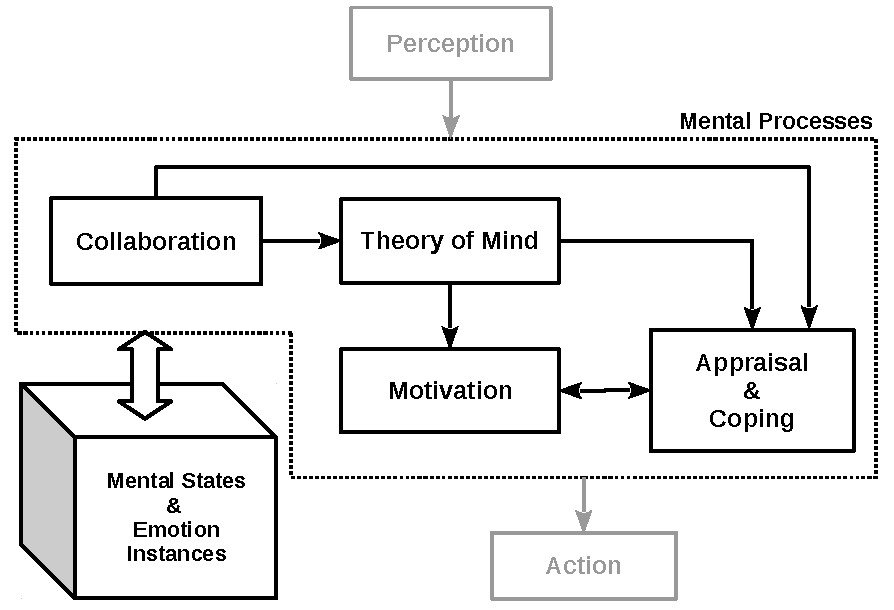
\includegraphics[scale=0.78]{figure/theory-general-croped.pdf}
  \caption{Computational framework based on \textit{Affective Motivational
  Collaboration Theory} (arrows indicate primary influences between
  mechanisms).}
  \label{fig:theory}
\end{figure}

In summary, Affective Motivational Collaboration Theory consists of five
mechanisms all of which store and retrieve data in the Mental States. We will
describe each mechanism and their influences on each other briefly below.

\subsection{Collaboration Mechanism}
\label{sec:collaboration-mech}

The \textit{Collaboration} mechanism (see Fig.~\ref{fig:theory}) constructs
a hierarchy of tasks and also manages and maintains the constraints and other
required details of the collaboration specified by the plan. These constraints
on task states and on the ordering of tasks include the inputs and outputs of
individual tasks, the preconditions specifying whether it is appropriate to
perform a task (which can be used as an indication of an impasse), and the
postconditions specifying whether a just-completed task was successful (or
failed). The Collaboration mechanism includes processes to update and monitor
the shared plan. It also keeps track of the focus of attention, which specifies
the salient objects, properties and relations at each point of the
collaboration. These processes depend on the operation of other mechanisms. For
instance, the Appraisal mechanism is required to evaluate the current mental
state with respect to the current status of the collaboration. Also, the
Appraisal and Motivation mechanisms provide interpretation of task failure and
the formation of a new mental state (e.g.\,an intention) respectively.

\subsection{Appraisal \& Coping Mechanisms}
\label{sec:appraisal-coping-mech}

Appraisal is a subjective evaluation mechanism based on individual processes
each of which computes the value of the appraisal variables. The Appraisal
mechanism is responsible for evaluating changes in the Robot's mental state, the
anticipated mental state of the human, and the state of the collaboration
environment. Collaboration requires the evaluative function of the Appraisal
mechanism for various reasons. The course of a collaboration is based on a full
or a partial plan \cite{grosz:collaboration,grosz:discourse-structure} which
needs to be updated as time passes and collaborators achieve, fail at or abandon
a task assigned to them. The failure of a task should not destroy the entire
collaboration. Appraising the environment and the current event helps the Robot
to update the collaboration plan in response to changes in the environment and
avoid further critical failures during collaboration. Appraisal also helps the
Robot to have a better understanding of the human's actions by making inferences
based on appraisal variables (see Section \ref{sec:wtce} for some examples)
\cite{marsella:ema-process-model} \cite{scherer:appraisal-processes}.
Furthermore, in order to collaborate successfully, a collaborator cannot simply
use the plan and reach to the shared goal; there should be an adaptation
mechanism not only for updating the plan but also the underlying mental state.
The output of Appraisal can directly and indirectly impact other mechanisms. For
instance, the Motivation mechanism uses this data to generate, compare and
monitor motives based on the current internal appraisal of the Robot as well as
the appraisal of the environment.

The Coping mechanism is responsible for adopting the appropriate behavior
(action) with respect to interpretation of the ongoing internal and external
changes. The Coping mechanism provides the Robot with different coping
strategies associated with changes in the Robot's mental state with respect to
the state of the collaboration. In other words, the Coping mechanism produces
cognitive responses based on the appraisal patterns.

\subsection{Motivation Mechanism}
\label{sec:motivation-mech}

The \textit{Motivation} mechanism operates whenever the Robot a) requires a new
motive to overcome an internal impasse in an ongoing task, or b) wants to
provide an external motive to the human when the human faces a problem in a
task. In both cases, the Motivation mechanism uses the Appraisal mechanism to
compute attributes of the competing motives. The purpose of Motivation mechanism
in Affective Motivational Collaboration Theory is to generate new emotion-driven
goal-directed motives considered as ``potential'' intentions. These motives are
generated based on what the Robot believes about the environment including the
Robot and the other collaborator and the corresponding appraisals. The Robot
uses these motives to reach to a private or shared goal according to new
conditions caused by changes in the environment. The Motivation mechanism
consists of an arrangement of three distinct processes. First, several motives
are generated with respect to the current mental state. Only one of these
competing motives is most likely to become a new intention. Therefore, a
comparison process decides which motive is more likely to be consistent with the
current state based on the values of the motive attributes (e.g., motive
insistence and motive urgency). Finally, the new motive will be used to form a
new intention. As a result, the Robot can take an action based on the new
intention to sustain the collaboration progress. Furthermore, the Motivation
mechanism can serve the Theory of Mind mechanism by helping the Robot to infer
the motive behind the human's current action.

\subsection{Theory of Mind Mechanism}
\label{sec:tom-mech}

The \textit{Theory of Mind} mechanism is the mechanism for inferring a model of
the human's anticipated mental state. The Robot uses the Theory of Mind
mechanism to infer and attribute beliefs, intentions, motives and goals to its
collaborator based on the user model it creates and maintains during
collaboration. The Robot progressively updates this model during the
collaboration. The refinement of this model helps the Robot to anticipate the
human's mental state more accurately, which ultimately impacts the quality of
the collaboration and the achievement of the shared goal. Furthermore, the Robot
can make inferences about the motive (or intention) behind the human's actions
using the Motivation mechanism. This inference helps the Robot to update its own
beliefs about the human's mental state. In the reverse appraisal process
\cite{gratch:reverse-appraisal}, the Robot also applies the Appraisal mechanism
together with updated beliefs about the human's Mental States to infer the
human's current mental state based on the human's emotional expression. Finally,
the Collaboration mechanism provides the collaboration structure, including
status of the shared plan with respect to the shared goal and the mutual beliefs
to the Theory of Mind mechanism. Consequently, any change to the Robot's model
of the human will update the Robot's mental state.

\subsection{Perception \& Action}
\label{sec:tom-mech}

Perception is outside of our theory and is responsible for producing the sensory
information used by the mechanisms in our framework; it is only a source of data
to the computational framework (see Fig.\,\ref{fig:theory}). Thus, our
computational framework starts with high-level semantic representation of events
(including utterances). The output of the Perception component provides a
unified perception representation across all of the mechanisms.

The Action component in Fig.\,\ref{fig:theory}, which is also outside of our
theory, functions whenever the Robot needs to show a proper behavior according
to the result of the internal processes of the collaboration procedure; it is
only a sink of data in our computational framework. The only input to the Action
component is provided by the Coping mechanism. This input will cause the Action
component to execute an appropriate behavior of the Robot. This input to Action
has the same level of abstraction as the output of the Perception mechanism,
i.e., it includes the Robot's utterances, primitive actions and emotional
expressions.

\subsection{Mental States \& Emotion Instances}

The Mental States shown in Fig.\,\ref{fig:theory} comprise the knowledge base
required for all the mechanisms in the overall framework.

\subsubsection{Beliefs}
\label{sec:beliefs}

\textit{Beliefs} are a crucial part of the Mental States. We have two different
perspectives on categorization of beliefs. In one perspective, we categorize
beliefs based on whether or not they are shared between the collaborators. The
SharedPlans \cite{grosz:plans-discourse} theory is the foundation of this
categorization in which for any given proposition the Robot may have: a) private
beliefs (the Robot believes the human does not know these), b) the inferred
beliefs of the human (the Robot believes the human collaborator has these
beliefs), and c) mutual beliefs (the Robot believes both the Robot and the human
have these same beliefs and both of them believe that). From another
perspective, we categorize beliefs based on who or what they are about. In this
categorization, beliefs can be about the Robot, the human, or the environment.
Beliefs about the environment can be about internal events, such as outcomes of
a new appraisal or a new motive, or external events such as the human's offer,
question or request, and general beliefs about the environment in which the
Robot is situated. Beliefs can be created and updated by different processes.
They also affect how these processes function as time passes.

\subsubsection{Intentions}
\label{sec:intentions}

\textit{Intentions} are mental constructs directed at future actions. They play
an essential role in: a) taking actions according to the collaboration plan, b)
coordination of actions with the human collaborator, c) formation of beliefs
about the Robot and anticipated beliefs about the human, and d) behavior
selection in the Coping mechanism. First, taking actions means that the Robot
will intend to take an action for primitive tasks that have gained the focus of
attention, possess active motives, and have satisfied preconditions for which
required temporal predecessors have been successfully achieved. Second,
intentions are involved in action coordinations in which the human's behavior
guides the Robot to infer an anticipated behavior of the human. Third,
intentions play a role in belief formation, mainly as a result of the permanence
and commitment inherent to intentions in subsequent processes, e.g., appraisal
of the human's reaction to the current action and self-regulation. Lastly,
intentions are involved in selecting intention-related strategies, e.g.,
planning, seeking instrumental support and procrastination, which are an
essential category of the strategies in the Coping mechanism
\cite{marsella:ema-process-model}. Intentions possess a set of attributes, e.g.
\textit{involvement, certainty, ambivalence} which moderate the consistency
between intention and behavior. The issue of consistency between the intentions
(in collaboration) and the behaviors (as a result of the Coping mechanism in the
appraisal cycle) is important because neither of these two mechanisms alone
provides solution for this concern.

\subsubsection{Motives}
\label{sec:motives}

\textit{Motives} are emotion-driven goal-directed mental constructs which can
initiate, direct and maintain goal-directed behaviors. They are created by the
emotion-regulated Motivation mechanism. Motives can cause the formation of a new
intention for the Robot according to: a) its own emotional states (how the Robot
feels about something), b) its own private goal (how an action helps the Robot
to make progress), c) the collaboration goal (how an action helps to achieve the
shared goal), and d) the human's anticipated beliefs (how an action helps the
human). Motives also possess a set of attributes, e.g., \textit{insistence} or
\textit{failure disruptiveness}. These attributes are involved in the comparison
of newly generated motives based on the current state of the collaboration.
Ultimately, the Robot forms or updates an intention about the winning motive in
the Mental States.

\subsubsection{Goals}
\label{sec:goals}

\textit{Goals} help the Robot to create and update the structure of the
collaboration plan. Goals direct the formation of intentions to take appropriate
corresponding actions during collaboration. Goals also drive the Motivation
mechanism to generate required motive(s) in uncertain or ambiguous situations,
e.g., to minimize the risk of impasse or to reprioritize goals. Goals have
three attributes. The \textit{specificity} of goals has two functions for the
Robot. First, it defines the performance standard for evaluating the progress
and quality of the collaboration. Second, it serves the Robot to infer the
winner of competing motives. The \textit{proximity} of goals distinguishes goals
according to how ``far'' they are from the ongoing task. Proximal (or
short-term) goals are achievable more quickly, and result in higher motivation
and better self-regulation than more temporally distant (or long-term) goals.
Goals can influence the \textit{strength} of beliefs, which is an important
attribute for regulating the elicitation of social emotions. The
\textit{Difficulty} of goals impacts collaborative events and decisions in the
appraisal, reverse appraisal, motive generation and intention formation
processes. For instance, overly easy goals do not motivate; neither are humans
motivated to attempt what they believe are impossible goals.

\subsubsection{Emotions}

\textit{Emotions} in Mental States are emotion instances that are elicited by
the Appraisal mechanism. These emotion instances include the Robot's own
emotions as well as the anticipated emotions of the human which are created with
the help of the processes in the Theory of Mind mechanism.

\section{Computational Walkthroughs}
\label{sec:wtce}

In this section, we explain in detail how the individual computational
mechanisms described in Section \ref{sec:computational-framework} generate the
Robot's behaviors in each example in Section \ref{sec:example-scenario}. The
following four walkthrough examples are in the same order as the four examples
in Section \ref{sec:example-scenario}. The name of the mechanisms written in
parantheses and bold indicates below which mechanism is involved in each step.
There are also specific processes written after a colon in front of the
mechanism, if appropriate.

\subsection{Agreeing on Shared Goal (Emotion-Awareness)}
\label{sec:wt-exp1}

This section provides a step-by-step walkthrough explanation of the example
presented in Section \ref{sec:exp1}. In this example, the explanation between
Astronaut's utterance A1 and Robot's utterance A2 illustrates how the Robot
perceives and interprets events including Astronaut's utterances and emotional
expressions, and how the Robot takes an appropriate action whenever it is
required.\footnote{Since our walkthrough explanation of underlying processes is
based on collaborators' utterances, we use \textbf{verbal} expression of
emotions within the utterances to emphasize their existence in certain parts of
the collaboration. However, although the nonverbal emotional expressions (e.g.,
facial expressions) can provide the same impact during collaboration, the
automatic recognition of them is out of our research context.}\\

\noindent\fbox{\begin{varwidth}{0.98\textwidth}
\textit{\textbf{\fontsize{9pt}{12pt}\selectfont{A1. Astronaut:}}} Oh no!
Finishing the quality check of our installation with this measurement problem is
so frustrating. I think we should stop now!\end{varwidth}}\\ \\

%\fontsize{9pt}{10pt}\selectfont
\noindent \textbf{(Perception)} The Robot perceives the Astronaut's utterances
and emotion.\\
  
First, the Robot perceives the Astronaut's utterances as well as her emotion in
the first turn (A1). The output of Perception is beliefs about the task in the
Astronaut's focus of attention, and also the Astronaut's emotion which she has
expressed both verbally and nonverbally. The beliefs formed about the task
(i.e., installing the panel) include:

\begin{itemize}
  \item[$\bullet$] the Astronaut's proposal of \textit{stopping} the task,
  \item[$\bullet$] which is a \textit{future} event,
  \item[$\bullet$] and is \textit{caused by} the measurement tool problem.
\end{itemize}

\noindent Also, beliefs formed about the Astronaut's emotion (i.e., frustration)
include:

\begin{itemize}
  \item[$\bullet$] the existence of a \textit{negative-valenced} emotion,
  \item[$\bullet$] and is verbally conveyed as \textit{frustration}.\\
\end{itemize}

\noindent\textbf{(Collaboration: \textit{Monitoring \& Focus Shifting})}
Based on these perceptions, the Robot uses the Collaboration mechanism, and
forms new beliefs about the collaboration status. These new beliefs are about:

\begin{itemize}
  \item[$\bullet$] the \textit{unsatisfied} precondition of the Astronaut's
  current \textit{task},
  \item[$\bullet$] the \textit{blocked} status of the Astronaut's current
  \textit{task},
  \item[$\bullet$] and consequently the \textit{blocked} status of the
  \textit{shared goal},
  \item[$\bullet$] which causes the change in the Robot's \textit{focus of
  attention} to the Astronaut's task.
\end{itemize}

\noindent \textbf{(Theory of Mind: \textit{Reverse Appraisal \& User
Modeling})} The Robot uses reverse appraisal to understand the meaning of the
Astronaut's frustration according to the collaborative task status (e.g.,
precondition and shared goal status). The Robot updates the Astronaut's user
model correspondingly.\\

The reverse appraisal process forms beliefs about the anticipated appraisals of
the Astronaut with respect to the current task's status based on the Astronaut's
utterances and emotion in A1, and the output of the collaboration mechanism.
Some of these anticipated appraisal values indicate that the event is
interpreted as \textit{relevant}, \textit{undesirable}, \textit{uncontrollable},
\textit{urgent}, and \textit{unexpected} by the Astronaut. Furthermore, the user
modeling process updates the Astronaut's user model based on the output of the
reverse appraisal process and the collaboration mechanism; this user modeling
process forms beliefs that:

\begin{itemize}
  \item[$\bullet$] Astronaut has \textit{low autonomy},
  \item[$\bullet$] Astronaut is a \textit{highly communicative} collaborator.
\end{itemize}

\noindent \textbf{(Appraisal)} The Robot appraises the Astronaut's utterances
and emotion.\\

The Appraisal mechanism simultaneously uses distinct processes to compute values
for each individual appraisal variable. The output of these processes provides a
vector of values describing the Robot's interpretation of the current event
(A1). In this example, the beliefs listed above including the negative-valenced
emotion provide a vector of values that would be read as frustration. The Action
component has the task of expressing this emotion.\\

\noindent \textbf{(Motivation: \textit{Motive \& Intention Formation})}
The Robot forms new motives according to the result of:

\begin{enumerate}[a)]
  \item appraisal with respect to the shared goal,
  \item reverse appraisal of the Astronaut's emotion,
  \item and the user model of the Astronaut. 
\end{enumerate}

Then, the motive comparison process compares current available motives and
sorts them based on their distance to the Astronaut's emotional state and
the achievement of the shared goal. Here, the distance function is a function of
a) the Astronaut's emotional state as an admissible approximation of her mental
state, and b) how taking an action based on the corresponding intention of a
particular motive improves the possibility of the collaborators reaching to the
collaborators' mutually accepted shared goal. The Robot ultimately selects the
most related motive and forms a new intention with respect to the current status
of collaboration. After this whole process, the Robot uses the coping mechanism
to take an action based on the available intention.\\

\noindent \textbf{(Coping)} Based on the current mental state, the Robot chooses
an emotion-focused coping strategy, decides to acknowledge the Astronaut's
emotion, and to provide an alternative solution. Subsequently, the Robot
responds to the Astronaut with A2.\\

\noindent \fbox{\begin{varwidth}{0.98\textwidth}
\textit{\textbf{\fontsize{9pt}{12pt}\selectfont{A2. Robot:}}} I see. This is
frustrating. But, I can help you with the measurement tool and we can finish the
task as originally planned. \end{varwidth}}\\

The Astronaut's new utterance (A3) provides the Robot with a new question about
whether the Robot can fix the measurement tool. The following paragraphs show
how the robot employs the same mechanisms described in Section
\ref{sec:computational-framework} to negotiate with the Astronaut to reach an
agreement on the shared goal.\\

\noindent\fbox{\begin{varwidth}{0.98\textwidth}
\textit{\textbf{\fontsize{9pt}{12pt}\selectfont{A3. Astronaut:}}} Can you fix
the measurement tool?\end{varwidth}}\\

Using the same processes as before, the following beliefs hold:

\begin{itemize}
  \item[$\bullet$] the precondition associated with the Astronaut's current
  \textit{task} is still \textit{unsatisfied},
  \item[$\bullet$] the status of the Astronaut's current \textit{task} is still
  \textit{blocked},
  \item[$\bullet$] and similarly the status of the \textit{shared goal} is
  still \textit{blocked},
  \item[$\bullet$] however, the Astronaut's question changes the Robot's
  \textit{focus of attention} to the measurement tool,
  \item[$\bullet$] also, the Astronaut's \textit{emotion} has changed to
  \textit{neutral}.
  \item[$\bullet$] but, her user model \textit{stays the same}, i.e.,
  having low-autonomy and being highly communicative.
\end{itemize}

\noindent\textbf{(Collaboration)} The change in the focus of attention to the
measurement tool causes the Robot to check the availability of a recipe to fix
or replace the malfunctioning measurement tool. The Robot finds a recipe to
replace the measurement tool.\\

\noindent\textbf{(Appraisal)} The Robot appraises the possibility of
replacing the measurement tool with respect to: a) the status of the shared
goal, and b) the Astronaut's user model. Robot finds the replacement of the
measurement tool \textit{relevant}, \textit{desirable}, and
\textit{controllable}.\\

\noindent\textbf{(Motivation: \textit{Motive \& Intention Formations})} The
Robot forms new motives based on the next task according to the shared plan and
outcome of the appraisal of the possibility of replacing the measurement tool.
The Robot forms the corresponding intentions with respect to the new motives.\\

\noindent Once again, the Robot uses the coping mechanism to take an action
based on the recent intention.\\

\noindent\textbf{(Coping)} Based on the current mental state, Robot
chooses to negotiate and offer an alternative action to the Astronaut (A4).\\

\noindent\fbox{\begin{varwidth}{0.98\textwidth}
\textit{\textbf{\fontsize{9pt}{12pt}\selectfont{A4. Robot:}}} The next task is
fixing the panel and it requires you to prepare and attach the welding rod to
your welding tool. To save our time, I will fetch another measurement tool while
you are preparing your welding tool.\end{varwidth}}\\

At this point, Astronaut is content with the way Robot outlined the shared goal
and responds respectively (A5). The Robot perceives and interprets the
Astronaut's response as an agreement on their new shared goal as we discussed
above.\\

\noindent\fbox{\begin{varwidth}{0.98\textwidth}
\textit{\textbf{\fontsize{9pt}{12pt}\selectfont{A5. Astronaut:}}} That would be
great!\end{varwidth}}

\subsection{Agreeing on Shared Goal (Emotion-Ignorance)}
\label{sec:wt-exp2}

This walkthrough example begins with the same utterance as the previous one, and
it provides the computational walkthrough of the emotional-ignorance example in
Section \ref{sec:exp2}. In emotional-ignorance examples, we assume Robot always
perceives neutral emotion expressed by the Astronaut. To avoid redundant
explanations, we refer to similar processing in the previous walkthrough
example, when possible.\\

\noindent\fbox{\begin{varwidth}{0.98\textwidth}
\textit{\textbf{\fontsize{9pt}{12pt}\selectfont{B1. Astronaut:}}} Oh no!
Finishing the quality check of our installation with this measurement problem is
so frustrating. I think we should stop now!\end{varwidth}}\\

\noindent\textbf{(Perception)} The Robot only perceives the Astronaut's
utterances (B1).\\

Here, in the first step, the Robot perceives the Astronaut's utterances and
ignores her expressed emotion in B1, i.e., frustration. Similarly to the
previous example, Perception forms beliefs about the task in the Astronaut's
focus of attention. These beliefs include:

\begin{itemize}
  \item[$\bullet$] the Astronaut's proposal of \textit{stopping} the task,
  \item[$\bullet$] which is a \textit{future} event,
  \item[$\bullet$] and is \textit{caused by} the measurement tool problem.
\end{itemize}

\noindent Notice that beliefs about the Astronaut's emotion are formed
differently in comparison with the previous example, and are based on the
neutral emotion of the Astronaut, since the Robot ignores the Astronaut's actual
emotion instance, i.e., frustration. These beliefs include:

\begin{itemize}
  \item[$\bullet$] the existence of a \textit{neutral valenced} emotion,
  \item[$\bullet$] which maps into a three-value vector of \textit{pleasure},
  \textit{arousal}, and \textit{dominance},
  \item[$\bullet$] and is verbally conveyed as \textit{neutral} emotion.\\
\end{itemize}

\noindent\textbf{(Collaboration)} The Robot uses the collaboration mechanism to
form new beliefs about the collaboration status based on its perception. These
new beliefs are the same as those generated by Collaboration mechanism in the
previous example.\\

\noindent\textbf{(Theory of Mind: \textit{Reverse Appraisal \& User Modeling})}
The Robot uses reverse appraisal to understand the meaning of the Astronaut's
neutral emotion according to the collaborative task status (e.g., precondition
and shared goal status). The Robot updates the Astronaut's user model
respectively.\\

In this example, since the Robot misses the actual expressed emotion by the
Astronaut (i.e., frustration) and incorrectly perceives her with neutral
emotion, the corresponding anticipated appraisal values lead to the wrong
interpretation of the event. The Robot thinks the Astronaut interprets the
event as \textit{desirable}, \textit{controllable}, \textit{non-urgent}, and
\textit{expected} (all of which are incorrect). Furthermore, the user modeling
process forms incorrect beliefs:

\begin{itemize}
  \item[$\bullet$] Astronaut has \textit{high autonomy},
  \item[$\bullet$] Astronaut is a \textit{moderately communicative}
  collaborator.
\end{itemize}

\noindent\textbf{(Appraisal)} The Robot appraises the Astronaut's utterances.\\

The Appraisal mechanism operates similarly to what we discussed in Section
\ref{sec:exp1}. The output of these processes provides a vector of values
describing the Robot's interpretation of the current event (B1). The outcome
will also be mapped to a particular emotion instance, but since the Robot misses
Astronaut's emotion, it maps the appraisals to a different emotion, i.e.,
hope, than the one elicited in previous example. The Robot elicits hope because
it believes the Astronaut's emotion is neutral and the current task is blocked.
Therefore, the Robot wants to come up with an alternative solution
immediately.\\

\noindent\textbf{(Motivation: \textit{Motive \& Intention Formation})} As
we discussed earlier, the Robot forms new motives according to the result of:

\begin{enumerate}[a)]
  \item appraisal with respect to the shared goal,
  \item reverse appraisal of the Astronaut's emotion,
  \item and the user model of the Astronaut. 
\end{enumerate} 

Although the process of comparing and sorting available motives here is similar
to the previous example, all of the new motives are different. The reason is
that each of the above three sources of motives forms a different motive because
it holds a different value, which is caused by the ignorance of the Astronaut's
actual emotion. For instance, the motive generated with the influence of
appraisal in the emotional-awareness example urges the Robot to postpone asking
questions about the alternative solutions while the motive with the same cause
(i.e., appraisal) in emotional-ignorance example urges the Robot to immediately
try to fix the problem and come up with alternative solutions by asking
questions. The Robot, similarly to the previous example, selects the most
related motive and forms a new intention with respect to the current status of
collaboration. After this whole process, the Robot uses the coping mechanism to
take an action based on the available intention.\\

\noindent\textbf{(Coping)} Based on the current mental state, the Robot decides
to use a problem-focused coping strategy of seeking information to be able to
choose between two available actions and reduce the current amount of
uncertainty. Therefore, the Robot, without acknowledging the Astronaut's
emotion, asks the Astronaut to choose between two alternative solutions (B2).\\

\noindent\fbox{\begin{varwidth}{0.98\textwidth}
\textit{\textbf{\fontsize{9pt}{12pt}\selectfont{B2. Robot:}}} I can help you
with the measurement tool, or we can terminate this task.
What do you want me to do?\end{varwidth}}\\

As we mentioned earlier in Section \ref{sec:exp2}, the Robot's response does not
make any progress in the collaboration status. Hence, the Astronaut repeats
herself about the task status (B3).\\

\noindent\fbox{\begin{varwidth}{0.98\textwidth}
\textit{\textbf{\fontsize{9pt}{12pt}\selectfont{B3. Astronaut:}}} As I said the
measurement tool does not work properly. We can not continue! \end{varwidth}}\\

The Robot perceives the Astronaut's new utterance (B3) while, again, ignoring
her frustration. The Robot goes through the same process as we described above,
and since the Astronaut has just repeated herself, her new utterances do not
change the Robot's mental state. Having the same mental state causes the Robot
to ask a similar question (B4).\\

\noindent\fbox{\begin{varwidth}{0.98\textwidth}
\textit{\textbf{\fontsize{9pt}{12pt}\selectfont{B4. Robot:}}} Okay. Do you want
me to fix this problem or terminate the task?\end{varwidth}}\\

This time, Robot's question makes an ambiguous assumption for the Astronaut on
whether the Robot can fix the disfunctional measurement tool for her. The
ambiguity of Robot's question does not help Astronaut's frustration and causes
her to ask a clarification question (B5).\\

\noindent\fbox{\begin{varwidth}{0.98\textwidth}
\textit{\textbf{\fontsize{9pt}{12pt}\selectfont{B5. Astronaut:}}} Can you fix my
measurement tool?\end{varwidth}}\\

Again, the same processes will be run (similar to what we had above) to form
beliefs for the new utterance of the Astronaut (B5) before the procedure that
follows. The new beliefs based on the Astronaut's new utterance are as follows.
Notice that the Robot still believes that the Astronaut's emotion is neutral.

\begin{itemize}
  \item[$\bullet$] the precondition associated to the Astronaut's current
  \textit{task} is still \textit{unsatisfied},
  \item[$\bullet$] the status of the Astronaut's current \textit{task} is still
  \textit{blocked},
  \item[$\bullet$] and similarly the status of the \textit{shared goal} is
  still \textit{blocked},
  \item[$\bullet$] however, the Astronaut's question changes the Robot's
  \textit{focus of attention} to fixing the measurement tool,
  \item[$\bullet$] also, the Astronaut's \textit{emotion} is still
  \textit{neutral}.
  \item[$\bullet$] but, her user model \textit{has changed} to having
  medium-autonomy and being highly communicative.
\end{itemize}

\noindent\textbf{(Collaboration)} The change in the focus of attention to fixing
the measurement tool causes the Robot to check the availability of a recipe to
fix or replace the disfunctioning measurement tool. Similarly to the previous
example, the Robot finds a recipe to replace the measurement tool.\\

\noindent\textbf{(Appraisal)} The Robot appraises the possibility of replacing
the measurement tool with respect to: a) the status of the shared goal, and b)
the Astronaut's user model. The Robot finds the replacement of the measurement
tool \textit{relevant}, \textit{desirable}, and \textit{controllable} just as
before.\\

\noindent\textbf{(Motivation: \textit{Motive \& Intention Formations})} The
Robot forms new motives based on the next task according to the shared plan and
the outcome of the appraisal of the possibility of replacing the measurement
tool. The Robot forms the corresponding intentions with respect to the new
motives.\\

\noindent Once again, the Robot decides to take an action based on the recent
intention.\\

\noindent\textbf{(Coping)} Based on the current mental state, first, the Robot
responds to the Astronaut's question, and then, chooses to negotiate and offer
an alternative action to the Astronaut (B6).\\

\noindent\fbox{\begin{varwidth}{0.98\textwidth}
\textit{\textbf{\fontsize{9pt}{12pt}\selectfont{B6. Robot:}}} I cannot fix your
measurement tool, but I can fetch another one for you if you want?
\end{varwidth}}\\

The Astronaut's strong emotion, shortage of time, and the Robot's mismatching
answer to the Astronaut's assumption causes the Astronaut to reject the Robot's
proposal (B7).\\

\noindent\fbox{\begin{varwidth}{0.98\textwidth}
\textit{\textbf{\fontsize{9pt}{12pt}\selectfont{B7. Astronaut:}}} No, I don't
want another measurement tool! We don't have time for that!\end{varwidth}}\\

After perceiving the Astronaut's answer the Robot tries to negotiate (using the
same procedure as we discussed above) with the Astronaut to protect the
collaboration and the shared goal from failure. Therefore, the Robot asks about
the possibility of pursuing another task.\\

\noindent\fbox{\begin{varwidth}{0.98\textwidth}
\textit{\textbf{\fontsize{9pt}{12pt}\selectfont{B8. Robot:}}} Okay. You want me
to terminate this task. Terminating this task can influence the quality of
installation of this solar panel which can cause the mission to fail. Or, do you
want us to work on another task? This can help us to install the panel using
your welding tool, but I do not know whether the quality of our installation
will be acceptable.\end{varwidth}}\\

The Astronaut terminates the collaboration due to the lack of time and failure
in the Robot's collaborative behavior (B9).\\

\noindent\fbox{\begin{varwidth}{0.98\textwidth}
\textit{\textbf{\fontsize{9pt}{12pt}\selectfont{B9. Astronaut:}}} I told you we
have this problem and we should terminate the mission! We cannot continue
without the measurement tool!\end{varwidth}}\\

As shown in this example, ignoring the Astronaut's emotion, impacts the Robot's
perception and corresponding beliefs. The output of the Collaboration mechanism
remains unchanged in comparison with the emotional-awareness example which is a
crucial point in our first two examples. Although the collaboration mechanism
provides the required structural details of collaboration between the Robot and
the Astronaut, these structural details are not enough for saving a
collaboration from a failure. As we continue, we can see that ignoring the
actual emotion of the Astronaut causes misfunctioning of the processes in the
Theory of Mind mechanism, i.e., reverse appraisal and user modeling. Comparing
the result of these two processes with the results in the emotional-awareness
example shows the importance of correctly perceiving a collaborator's emotion.
This problem continues even with the Appraisal mechanism which maps the Robot's
interpretation of the environment to a wrong emotion. Consequently, all
sources of the motivation mechanism provide incorrect values which drastically
influence the formation of the underlying motives of the required intentions.
Finally, the coping mechanism operates based on wrong newly formed intentions
which leads to a totally different behavior of the Robot in comparison with the
same turn in the emotional-awareness example. The divergence of the Robot's
collaborative behavior from its successful path continues among the Robot and
the Astronaut's interaction which increases the required time for achieving the
shared goal, and perpetuates the negative feeling of the Astronaut. The Robot
also misses the right time to begin a negotiation process to save the
collaboration from failure. Therefore, it causes the Astronaut to reject the
Robot's proposal which again aggravates the Astronaut's negative emotion.
Consequently, the same collaboration fails even though that the Robot uses the
same computational mechanisms, as we showed above. In Sections \ref{sec:wt-exp3}
and \ref{sec:wt-exp4}, as another example of collaborative behavior, we are
going to show the importance of emotional-awareness and its underlying
computational mechanisms in a task delegation procedure.

\subsection{Task Delegation (Emotion-Awareness)}
\label{sec:wt-exp3}

This walkthrough example is focusing on the delegation of a task by the
Astronaut during collaboration (see also the example in Section \ref{sec:exp3}).
In this example, the explanation between the Astronaut's utterance C1 and the
Robot's utterance C2 provides the details of how different mechanisms discussed
in Section \ref{sec:computational-framework} are involved in making the Robot 
show collaborative behaviors in acceptance of a new delegated task. To avoid
redundant explanations, we refer to similar procedures in previous walkthrough
examples.\\

\noindent\fbox{\begin{varwidth}{0.98\textwidth}
\textit{\textbf{\fontsize{9pt}{12pt}\selectfont{C1. Astronaut:}}} I still have
some problems with attaching the first panel! We do not have enough time. You
should begin to install the second panel.\end{varwidth}}\\

\noindent\textbf{(Perception)} The Robot perceives the Astronaut's utterances
and emotion in C1.\\

The perception mechanism forms beliefs based on the Astronaut's utterances and
her emotion (i.e., worry) which she has expressed nonverbally. We have shown
some examples of the beliefs formed by the perception mechanism in the example
in Section \ref{sec:wt-exp1}.\\

\noindent\textbf{(Collaboration: \textit{Interruption \& Constraint
Management})} The Robot infers the interruption and uses the constraint
management process to retrieve required resources and preconditions. the Robot
also checks whether there is an available associated recipe for the delegated
task.\\

\noindent\textbf{(Theory of Mind: \textit{Reverse Appraisal \& User Modeling})}
The Robot uses reverse appraisal to understand the meaning of the Astronaut's
worry with respect to the collaborative task status retrieved in the previous
step (e.g., precondition status, postcondition status, required resources,
shared goal). the Robot also updates the Astronaut's user model and forms
beliefs that a) the Astronaut has \textit{high autonomy}, and b) Astronaut is a
highly communicative collaborator. We have discussed more details about reverse
appraisal and user modeling processes in our example in Section
\ref{sec:wt-exp1}.\\

\noindent\textbf{(Appraisal)} The Robot appraises the Astronaut's utterances and
emotion. The Robot interprets the Astronaut's utterances and emotional state as
a \textit{relevant}, \textit{unexpected}, \textit{undesirable}, \textit{urgent},
but \textit{controllable} event.\\

\noindent\textbf{(Motivation: \textit{Motive \& Intention Formations})} The
Robot forms new motives based on the result of the same processes we discussed
in Section \ref{sec:wt-exp1}, and compares the available motives in the same way
we discussed in that section. The Robot forms new intention(s) with respect to
the selected motive.\\

\noindent\textbf{(Coping)} Based on the current mental state, the Robot chooses
an emotion-focused coping strategy and decides to acknowledge the Astronaut's
emotion, and provide a proper response (C2) without asking questions about the
delegated task.\\

\noindent\fbox{\begin{varwidth}{0.98\textwidth}
\textit{\textbf{\fontsize{9pt}{12pt}\selectfont{C2. Robot:}}} Okay. Don't worry.
I can handle that.\end{varwidth}}\\

The Astronaut perceives Robot's acknowledgment of her emotion as well as the
Robot's positive response to the Astronaut's delegated task. The Astronaut knows
that the Robot needs her to help with some of the primitive tasks in her own
delegated task to the Robot. Therefore, the Astronaut, while she is still
worried about time, informs the Robot that she will try to finish her current
task quickly.\\

\noindent\fbox{\begin{varwidth}{0.98\textwidth}
\textit{\textbf{\fontsize{9pt}{12pt}\selectfont{C3. Astronaut:}}} I will try to
fix it asap.\end{varwidth}}\\

The Robot perceives Astronaut's utterance and emotional expression. The same
process happens from updating beliefs to taking actions as we discussed above or
in previous examples. Since the Robot believes that the Astronaut is still
worried about time, it only informs the Astronaut about some potential questions
in the future. The Robot knows about these questions since there is either
missing information according to the partial plan, or required resources and
sub-tasks that can be provided by the Astronaut. The Robot chooses a proper
utterance about missing information according to the human's emotion (C4).\\

\noindent\fbox{\begin{varwidth}{0.98\textwidth}
\textit{\textbf{\fontsize{9pt}{12pt}\selectfont{C4. Robot:}}} I might need to
ask some questions while I am installing the second panel.\end{varwidth}}\\

The Astronaut finds the Robot's response appropriate for the delegated task.
Therefore, the Robot's proper response mitigates the Astronaut's negative
emotion which was caused by the lack of time for a successive installing
procedure of the first and second panels. As a result, the Astronaut properly
responds to the Robot's needs (C5).\\

\noindent\fbox{\begin{varwidth}{0.98\textwidth}
\textit{\textbf{\fontsize{9pt}{12pt}\selectfont{C5. Astronaut:}}} That's fine.
Just let me know.\end{varwidth}}

\subsection{Task Delegation (Emotion-Ignorance)}
\label{sec:wt-exp4}

This walkthrough example begins with the same exact utterance as the previous
one in Section \ref{sec:wt-exp3}. This section briefly provides the
corresponding details of the emotional-ignorance example in Section
\ref{sec:exp4} which is focusing on the delegation of a task by the Astronaut during
collaboration. In this example, the explanation between the Astronaut's
utterance D1 and the Robot's utterance D2 provides some details to show that
even though the same mechanisms (discussed in Section
\ref{sec:computational-framework}) are used to make the Robot obtain
collaborative behaviors, ignoring the Astronaut's expressed emotion changes the
output of different computational mechanisms (see also Section
\ref{sec:wt-exp2}) which ultimately causes unsuccessful termination of the task
delegation process. To avoid redundant explanations, we group some of the
Astronaut and Robot's utterances which constitute the representation of
repetitive interaction between them. We also refer to similar procedures in
previous walkthrough examples.\\

\noindent\fbox{\begin{varwidth}{0.98\textwidth}
\textit{\textbf{\fontsize{9pt}{12pt}\selectfont{D1. Astronaut:}}} I still have
some problems with attaching the first panel! We do not have enough time. You
should begin to install the second panel.\end{varwidth}}\\

\noindent\textbf{(Perception)} The Robot only perceives the Astronaut's
utterances (D1). These beliefs are about the unsatisfied postcondition of the
first task, i.e., installing the first solar panel, and the Astronaut's proposal
of installing the second panel. We have shown some examples of the beliefs
formed by perception mechanism in Section \ref{sec:wt-exp1}. Also, as we have
shown in Section \ref{sec:wt-exp2} that the Robot does not perceive the
Astronaut's emotion (i.e., worry). Therefore, the Robot misses beliefs about the
Astronaut's emotion.\\

\noindent\textbf{(Collaboration: \textit{Interruption \& Constraint
Management})} The Robot infers the interruption and uses the constraint
management process to retrieve required resources, and preconditions. Similarly
to the previous example, the Robot also checks whether there is an available
associated recipe for the delegated task. Ignoring the Astronaut's expressed
emotion does not change the beliefs formed based on the output of the
collaboration mechanism.\\

\noindent\textbf{(Theory of Mind: \textit{Reverse Appraisal \& User Modeling})}
Similar to the example in Section \ref{sec:wt-exp2}, the Robot uses reverse
appraisal to understand the meaning of the Astronaut's emotion with respect to
the collaborative task status. However, since the Robot ignores the Astronaut's
actual emotion, the output of the reverse appraisal does not help the Robot's
inference about its own collaborative behavior (see Section \ref{sec:wt-exp2}).
Similarly, the Robot updates the Astronaut's user model based on wrong beliefs
achieved by ignoring the Astronaut's expressed emotion. We have discussed more
details about reverse appraisal and user modeling processes in our example in
Section \ref{sec:wt-exp1}, and we have shown similar effects in Section
\ref{sec:wt-exp2}.\\

\noindent\textbf{(Appraisal)} The Robot appraises the Astronaut's utterances
with a wrong assumption of her expressing neutral emotion. Consequently, similar
to the example in Section \ref{sec:wt-exp3}, the Robot interprets the
Astronaut's utterances as a \textit{relevant}, \textit{unexpected},
\textit{undesirable}, \textit{urgent}, and \textit{controllable} event.\\

\noindent\textbf{(Motivation: \textit{Motive \& Intention Formations})} The
Robot forms and compares new motives in the same way as we have discussed in
previous examples. However, both processes of the motive formation and
comparison are performed based on false outputs of the other processes (see also
Section \ref{sec:wt-exp2}). Therefore, the Robot forms a new intention with
respect to the selected motive which can be formed or selected for a wrong
reason.\\

\noindent\textbf{(Coping)} Based on the current mental state (including a
wrong intention), the Robot decides to use problem-focused coping strategy of
seeking social support (seeking information) to be able to drop the intention of
working on the same task as the Astronaut. Respectively, Robot asks a question
(D2).\\

\noindent\fbox{\begin{varwidth}{0.98\textwidth}
\textit{\textbf{\fontsize{9pt}{12pt}\selectfont{D2. Robot:}}} Okay. I can handle
that. Is it okay if I leave the current task though? \end{varwidth}}\\

The rest of the Robot's utterances from D4 to D10 shows that the Robot wants to
do planning in the most efficient manner possible by asking many questions about
missing information according to the shared plan. On the other hand, the
Astronaut who was worried about the lack of time since the beginning, tries to
succinctly respond the Robot and successfully delegate the task. However, the
Robot, by asking several questions instead of understanding the Astronaut's
mental state and accepting the delegated task, causes the Astronaut to quickly
become frustrated and express her frustration (D9).\\

\noindent\fbox{\begin{varwidth}{0.98\textwidth}
\textit{\textbf{\fontsize{9pt}{12pt}\selectfont{D3. Astronaut:}}} Yes, that's
fine. I can finish it on my own.\\

\noindent \textit{\textbf{\fontsize{9pt}{12pt}\selectfont{D4. Robot:}}} Okay.
But according to the plan, I need your help when we need to weld the panel. Will
you be able to help me?\\

\noindent \textit{\textbf{\fontsize{9pt}{12pt}\selectfont{D5. Astronaut:}}} Yes,
I will.\\
  
\noindent \textit{\textbf{\fontsize{9pt}{12pt}\selectfont{D6. Robot:}}} We also
need your welding tool and supplies as well as the measuring tool to install the
second panel.\\
  
\noindent \textit{\textbf{\fontsize{9pt}{12pt}\selectfont{D7. Astronaut:}}} Just
let me know whenever you need something! \\
  
\noindent \textit{\textbf{\fontsize{9pt}{12pt}\selectfont{D8. Robot:}}} Thanks.
I will. How about the conflict that might occur while I am trying to fix the
second panel? You are going to need my help at the same time.\\
  
\noindent \textit{\textbf{\fontsize{9pt}{12pt}\selectfont{D9. Astronaut:}}}
Robot, I really don't understand what you are talking about!\\

\noindent \textit{\textbf{\fontsize{9pt}{12pt}\selectfont{D10. Robot:}}} Do you
want me to provide some examples? \end{varwidth}}\\

The Robot perceives the Astronaut's last utterance and once again ignores her
emotion. This time the Robot's tries to provide some examples to clarify its own
point which is another divergence from achieving the shared goal or planning for
the new delegated task (D10). Finally, the Astronaut terminates the
collaboration due to the lack of time and the Robot's failure in incorporating
proper collaborative behavior (D11).\\

\noindent\fbox{\begin{varwidth}{0.98\textwidth}
\textit{\textbf{\fontsize{9pt}{12pt}\selectfont{D11. Astronaut:}}} We don't have
time for this anymore! \end{varwidth}}

\section{Related Work}
\label{sec:related-work}

The prominent collaboration theories are mostly based on plans and joint
intentions
\cite{cohen:teamwork} \cite{grosz:plans-discourse}, and they were derived from
the BDI paradigm developed by Bratman \cite{bratman:intentions-plans} which is
fundamentally reliant on folk psychology \cite{ravenscroft:folk}. The two
theories, Joint Intentions \cite{cohen:teamwork} and SharedPlans
\cite{grosz:plans-discourse}, have been extensively used to examine and describe
teamwork and collaboration. There are many research focusing on different
aspects of collaboration based on different collaboration theories, i.e.,
SharedPlans
\cite{grosz:planning-acting,grosz:collaboration,grosz:plans-discourse}, Joint
Intentions \cite{cohen:teamwork}, and hybrid theories of collaboration, e.g.,
STEAM \cite{tambe:flexible-teamwork}. All of the works presented in this section
lack a systematic integration of collaboration theories with some theories
capable of describing underlying collaboration processes. Therefore, they either
do not explain the structure and the underlying processes of collaboration, or
their approach in either or both of these views is application oriented. In the
rest of this section, we provide a review of several applications of different
prominent collaboration theories which puts emphasis on the importance of the
collaborative robots and their applications. And at the end, we also provide
some related works on applications of artificial emotions and appraisal theory
to express the importance of their applicability in robots and autonomous
agents.

There are some works focusing on the concepts of robot assistants
\cite{clancey:agent-assistants-collaboration}, or teamwork and its challenges in
cognitive and behavioral levels
\cite{nikolaidis:collaboration-joint-action}
\cite{scerri:prototype-distributed-teams}. Some researchers have an overall look
at a collaboration concept at the architectural level. In
\cite{garcia:collaboration-emotional-awareness} authors present a collaborative
architecture, COCHI, and argue the need to support emotional-awareness in the
design and implementation of groupwares. In
\cite{esau:integrating-emotion-collaboration} authors present the integration of
emotional competence into a cognitive architecture which runs on a robot, MEXI.
In \cite{sofge:collaboration-humanoid-space} authors discuss the challenges of
integrating natural language, gesture understanding and spatial reasoning of a
collaborative humanoid robot situated in space. The importance of communication
during collaboration has also been considered by some researchers from
human-computer interaction and human-robot collaboration
\cite{clair:action-intention-collaboraiton}
\cite{matignon:verbal-nonverbal-collaboration} \cite{rich:discourse} to theories
describing collaborative negotiation, and discourse planning and structures
\cite{andriessen:disourse-planning} \cite{grosz:discourse-structure}
\cite{sidner:discourse-collaborative-negotiation}. There are other concepts such
as joint actions and commitments \cite{grosz:intention-dynamics-collaboration},
dynamics of intentions during collaboration \cite{levesque:acting-together}, and
task-based planning providing more depth in the context of collaboration
\cite{burghart:cognitive-architecture-robot} \cite{rich:cea}. The concept of
collaboration has also received attention in the industry and in research in
robotic laboratories \cite{green:collaboration-literature-review}. Some of these
works emphasize the applicability of emotions in their architectures, and some
others emphasize the collaborative aspect of their robots. In the following
pages, we review some of the applications of each prominent collaboration
theory.\\

\textbf{Collaboration Theories} -- COLLAGEN
\cite{rich:collaboration-manager,rich:discourse} is the first implemented system
based on the SharedPlans theory. It incorporates certain algorithms for
discourse generation and interpretation, and is able to maintain a segmented
interaction history, which facilitates the discourse between the human user and
the intelligent agent \cite{rickel:discourse-theory-dialogue}. In
\cite{lochbaum:plan-models}, Lochbaum and Sidner modify and expand the
SharedPlan model of collaborative behavior \cite{grosz:plans-discourse}. They
present an algorithm for updating an agent's beliefs about a partial shared plan
and describe an initial implementation of this algorithm in the domain of
network management. Lochbaum, also in \cite{lochbaum:collaborative-planning},
provides a computational model (based on the collaborative planning framework of
SharedPlans \cite{grosz:collaboration}) for recognizing intentional structure
and utilizing it in discourse processing. In short, she presents a SharedPlans
model for recognizing Discourse Segment Purposes (DSPs)
\cite{grosz:plans-discourse} \cite{sidner:discourse-collaborative-negotiation}
and their interrelationships. CAST (Collaborative Agents for Simulating
Teamwork) \cite{yen:cast} \cite{yin:knowledge-based-sharedplans} is a teamwork
framework based on the SharedPlans theory. CAST focuses on flexibility in
dynamic environments and on proactive information exchange enabled by
anticipating what information team members will need. Petri Nets are used to
represent both the team structure and the teamwork process, i.e., the plans to
be executed.

Breazeal et. al. in \cite{breazeal:humanoid-robots} present an overview of their
work towards building socially intelligent, cooperative humanoid robots,
Leonardo, that can collaborate and learn in partnership with humans. They employ
the Joint Intentions theory of collaboration to implement the collaborative
behaviors while performing a task in collaboration with humans. Mutlu et. al. in
\cite{mutlu:coordination-robot} discuss key mechanisms for effective
coordination toward informing the design of communication and coordination
mechanisms for robots. They present two illustrative studies that explore how
robot behavior might be designed to employ these mechanisms (particularly joint
attention and action observation) to improve measure of task performance in
human-robot collaboration. Their work uses Joint Intentions theory to develop
shared task representations and strategies for task decomposition. The domain
independent teamwork model, STEAM \cite{tambe:flexible-teamwork}, has also been
successfully applied to a variety of domains
\cite{kabil:coordination-mechanisms} \cite{kitano:robocup}
\cite{marsella:robocup} \cite{scerri:robot-agent-person}.\\

The applications of different prominent collaboration theories show the
importance and the applicability of these theories in robots and collaborative
systems. The following examples briefly review some of the applications of
artificial emotions and appraisal theory of emotions in robots and autonomous
agents.\\

\textbf{Artificial Emotions} -- There are many research areas, including
robotics and autonomous agents, that employ the structure and/or functions of
emotions in their work with a variety of motivations behind modeling emotions
\cite{wehrle:motivations-modeling-emotion}. Some of these works are inspired by
specific psychological theories, some are freely using the concept of emotion
without using the theoretical background in social sciences, and some are using
a combination of concepts from the psychological theories. For instance, in PECS
\cite{urban:pecs} which is designed for modeling human behaviors, the agent's
architecture is not based on a certain kind of social or psychological emotion
theory. The PECS' design enables an integrative modeling of physical, emotional,
cognitive and social influences within a component-oriented agent architecture.
Some researchers apply combinations of emotion theories in their work
\cite{kiryazov:modeling-appraisal-pad}. We can also see the application of
emotion theories in designing companion robots, robots capable of expressing
emotions and social behaviors, as well as robots which can convey certain types
of emotion products, e.g., empathy \cite{breazeal:expressive-behavior}
\cite{paiva:emotion-modeling} \cite{shayganfar:methodology}. Robots also use
emotions theories for for some other purposes such as automatic affect
recognition using different modalities \cite{zeng:affect-recognition}, and
behavior adaptation \cite{liu:affect-robot-behavior}.\\

\textbf{Appraisal Theory} -- Computational appraisal models have been applied to
a variety of uses including contributions to psychology, robotics, AI, and HCI.
For instance, Marsella and Gratch have used EMA
\cite{marsella:ema-process-model} to generate specific predictions about how
human subjects will appraise and cope with emotional situations and argue that
empirical tests of these predictions have implications for psychological
appraisal theory \cite{gratch:assessing-appraisal}. There are several examples
in artificial intelligence and robotics of applying appraisal theory
\cite{adam:bdi-emotional-companion} \cite{kim:model-hri-appraisal}
\cite{marsella:ema-process-model}. In robotics, appraisal theory has been used
to establish and maintain a better interaction between a robot and a human. For
instance in \cite{kim:model-hri-appraisal} researchers provide their
computational model of emotion generation based on appraisal theory to have a
positive human-robot interaction experience. In
\cite{sander:systems-approach-appraisal} authors describe a system approach to
appraisal processes based on Scherer's work on appraisal and the Component
Process Model \cite{scherer:nature-function-emotion}. They show how the temporal
unfolding of emotions can be experimentally tested. They also lay out a general
domain-independent computational model of appraisal and coping. In
\cite{vogiatzis:robot-museum} researchers consider their robot's (INDIGO)
emotion, speech and facial expressions as a key point to establish an effective
communication between the robot and a human during their interaction. They apply
concepts of appraisal theory in INDIGO's emotion modeling. MAGGIE, a sociable
robot, also applies the appraisal theory of emotions to consider fear in its
decision making system \cite{castro:autonomous-robot-fear}. Velasquez developed
Cathexis which is a distributed computational model for generation of emotions
and their influence in the behavior of the autonomous agents
\cite{velasquez:emotions-motivations-agents}. The emotion model in this work is
based on Roseman's work on appraisal theory. Marinier and Laird in
\cite{marinier:emotion-reinforcement} focus on the functional benefits of
emotion in a cognitive system. In this work, they integrate their emotion theory
(which is based on the appraisal theory) with Soar cognitive architecture, and
use emotional feedback to drive reinforcement learning. In
\cite{hudlicka:emotinos-reasons} Hudlicka provides a model of a generic
mechanism mediating the affective influences on cognition based on cognitive
appraisal. This model is implemented within a domain-independent
cognitive-affective architecture (MAMAID). In the virtual agents community,
empathy and affective decision-making is a research topic that has received much
attention in the last decade \cite{scott:modeling-empathy-agent}
\cite{paiva:agent-care} \cite{pontier:women-robot-men}.

\section{Conclusion and Future Work}

There is a correspondence between what a collaboration needs and what social
functions of emotions provide within a social context. In this paper, we argued
for the need of a theory explaining the underlying processes involved in a
collaboration. Then, we provided four hypothetical examples in two pairs. Each
pair of examples was about a distinct collaborative behavior. The first pair was
about agreeing on a shared goal between a robot and an astronaut, and the second
pair was about delegation of a new task to the robot by the astronaut. Each pair
of these examples contrasts a successful collaboration because the robot was
aware of the astronaut's emotion, and a failure in collaboration as the
consequence of the robot ignoring the astronaut's emotions. We provided a brief
description for each example as well as the utterances of both the robot and the
astronaut during their collaboration. These examples illustrated the importance
of emotional-awareness to attain successful collaborative behavior.

We also introduced the main components of Affective Motivational Collaboration
Theory as our computational framework which incorporates emotion-regulated
mechanisms, such as appraisal and coping, with collaboration processes, such as
planning, in a single unified framework. This framework let us describe the same
examples in more computational detail by explaining certain mechanisms and their
underlying processes, and how they are involved in helping the robot obtain a
collaborative behavior by observing the astronaut's emotions.

We have implemented the rules associated with these examples using JESS (Java
Expert System Shell) which is a rule engine for the Java platform. In our
current implementation we have categorized the rules in different modules
associated with the mechanisms and the underlying processes in \textit{Affective
Motivational Collaboration Thoery} (see Fig. \ref{fig:theory}). In our future
work, we will implement algorithms for each individual mechanism to be able to
automatically generate the required facts within each mechanism to fire the
existing rules. Ultimately, we are going to offer a platform which operates
based on the collaboration structure discussed by SharedPlans theory
\cite{grosz:discourse-structure}, and employs emotion-driven processes such as
the appraisal process in \cite{marsella:ema-process-model} to enable a robot to
obtain and demonstrate emotion-regulated collaborative behaviors.

%\label{sec:2} ~\ref{sec:1}

%\paragraph{Paragraph headings} 


% For one-column wide figures use
%\begin{figure}
% Use the relevant command to insert your figure file.
% For example, with the graphicx package use
%  
\includegraphics{example.eps}
% figure caption is below the figure
%\caption{Please write your figure caption here}
%\label{fig:1}       % Give a unique label
%\end{figure}
%
% For two-column wide figures use
%\begin{figure*}
% Use the relevant command to insert your figure file.
% For example, with the graphicx package use
%  
\includegraphics[width=0.75\textwidth]{example.eps}
% figure caption is below the figure
%\caption{Please write your figure caption here}
%\label{fig:2}       % Give a unique label
%\end{figure*}
%



% For tables use
%\begin{table}
% table caption is above the table
%\caption{Please write your table caption here}
%\label{tab:1}       % Give a unique label
% For LaTeX tables use
%\begin{tabular}{lll}
%\hline\noalign{\smallskip}
%first & second & third  \\
%\noalign{\smallskip}\hline\noalign{\smallskip}
%number & number & number \\
%number & number & number \\
%\noalign{\smallskip}\hline
%\end{tabular}
%\end{table}


%\begin{acknowledgements}
%If you'd like to thank anyone, place your comments here
%and remove the percent signs.
%\end{acknowledgements}

% BibTeX users please use one of
%\bibliographystyle{spbasic}      % basic style, author-year citations
%\bibliographystyle{spmpsci}      % mathematics and physical sciences
%\bibliographystyle{spphys}       % APS-like style for physics
%\bibliography{}   % name your BibTeX data base

% Non-BibTeX users please use
%\begin{thebibliography}{}
%
% and use \bibitem to create references. Consult the Instructions
% for authors for reference list style.
%
%\bibitem{RefJ}
% Format for Journal Reference
%Author, Article title, Journal, Volume, page numbers (year)

% Format for books

%\bibitem{RefB}
%Author, Book title, page numbers. Publisher, place (year)

% etc
%\end{thebibliography}

\bibliographystyle{abbrv}
\bibliography{mshayganfar.bib}

\end{document}
% end of file template.tex

